\question{Ein Pfeil wird auf eine Zielscheibe geschossen und bleibt stecken. Warum fliegt das Endstück Rückwärts weg?}

\begin{tasks}(1)
    \task[$\bullet$] Skizzieren Sie den Kraft- und Geschwindigkeitsverlauf im Pfeil (Dehnstab)
    \task[$\bullet$] Vergleichen sie Ihr Ergebnis mit einem Einmassenschwinger, der gegen die Wand fliegt.
\end{tasks}

\begin{solution}
\flushleft HIER BITTE NOCH LÖSUNG NACHTRAGEN (Dominik Kern)
\end{solution}

\question{Ein halbunendlicher Stab wird am Rand harmonisch angeregt.

\vspace{1cm}

\begin{figure}[h]
    \centering
    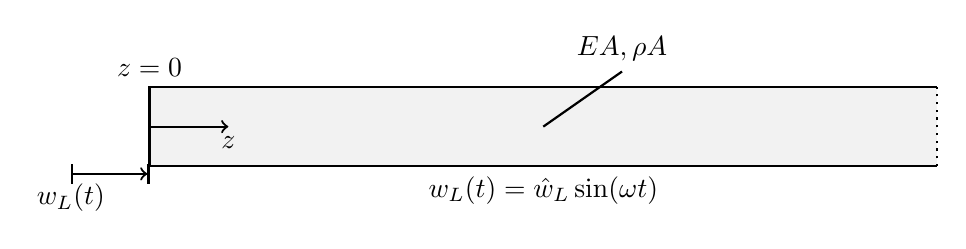
\begin{tikzpicture}
        \draw[thick, fill=gray!10] (10,0) -- node [midway, below] {$w_L (t) = \hat{w}_L \sin(\omega t)$} (0,0) -- (0,1) node[above] {$z=0$} -- (10,1) ;
        \draw[thick, dotted] (10,0) -- (10,1);
        %\draw[thick, ->] (10,0.5) -- (11,0.5);
        \draw[thick, ->] (0,0.5) -- (1,0.5) node[left, below] {$z$} ;
        \draw[thick, |->|] (-1,-0.1) node[below] {$w_L (t)$} -- (0,-0.10);
        \draw[thick] (5,0.5) -- (6,1.2) node[above] {$EA,\rho A$};
    \end{tikzpicture}
\end{figure}


Am Anfang $(t=0)$ ist er undeformiert und in Ruhe. Lösen Sie diese Aufgabe, indem Sie auf dem gedanklich über den Rand verlängerten Stab eine nach rechts laufende Welle annehmen, welche genau die vorgegebene Randbewegung erzeugt. Interpretieren Sie die Parameter dieses Verlaufs physikalisch, Stichwort ``Wellenlänge".
}

\begin{solution}
    
    \begin{align*}
        \intertext{Aus dem D'alembertschen Wellenansatz mit $t = 0$}
        &w_0(z) = \Psi(z) + \Phi(z)
        &\dot{w_0}(z) = c\Psi^{'}(z)-c\Psi^{'}(z)
        \intertext{folgt:}
        &\Psi(z) = C_1 \cos(\kappa z) + C_2 \sin(\kappa z)
        &\Phi(z) = R_1 \cos(\kappa z) + R_2 \sin(\kappa z)
    \end{align*}
\end{solution}

\question{Berechnen Sie das Reflektionsverhalten diskreter Elemente am Rand: Feder, Dämpfer und Masse.
\begin{figure}[h]
    \centering
    \begin{tikzpicture}

    \end{tikzpicture}
\end{figure}

\todo{Bilder einfügen}

Nehmen Sie dazu eine einfallende nach links laufende Welle $w_{ein}(z,t) = C_1 \cos(kz+\omega t)$ an und berechnen Sie die reflektierende Welle $w_{ref}(z,t)=R_1\cos(kz-\omega t) + R_2 \sin(kz-\omega t)$.
}\\[2em]

\fbox{Hinweis ($z=0$):}
\begin{tasks} (3)
    \task[] $kw = EAw'$
    \task[] $c\dot w = (EA)w'$
    \task[] $m\ddot w = (EA)w'$
    \task[] Feder-RB
    \task[] Dämpfer-RB
    \task[] Masse-RB
\end{tasks}

\fbox{Hinweis: Der Punkt steht für die Ableitung nacht, der Apostroph für die Ableitung nach z}

\begin{solution}
    \begin{align*}
        \intertext{Für Federn gilt:}
        &0 = kw - EA  w^{'}
        &R_1 = \frac{C_1 {(EA)}^2 \kappa^2 - C_1 k^2 + 2C_2 (EA) k \kappa}{{(EA)}^2 \kappa^2 + k^2}
        &R_2 = \frac{2C_1 (EA) k \kappa - C_2 {(EA)}^2 \kappa^2 + C_2 k^2}{{(EA)}^2 \kappa^2 + k^2}

        \intertext{Für Dämpfer gilt:}
        &0= c \dot{w} - EA  w^{'}
        &R_1 = \frac{C_1 (EA) \kappa - C_1 c w}{(EA) \kappa + cw}
        &R_2 = \frac{-C_2 (EA) \kappa + C_2 cw}{(EA) \kappa + cw}

        \intertext{Für die masse gilt:}
        &0 = m \ddot{w} - (EA) w^{'}
        &R_1 = \frac{C_1 {(EA)}^2 \kappa^2 - C_1 m^2 \omega^4 - 2C_2 (EA) \kappa m \omega^2}{{(EA)}^2 \kappa + m^2 \omega^4}
        &R_2 = \frac{-2C_1 (EA) \kappa m \omega^2 - C_2 {(EA)}^2 \kappa^2 + C_2 m^2 \omega^4}{{(EA)}^2 \kappa + m^2 \omega^4}
    \end{align*}
\end{solution}

\question{Resonant Column}

\vspace{1cm}

\begin{tikzpicture}
\draw[thick, fill=black!10!white] (-0.2, 0) rectangle (0.2, 3.0);
\draw[thick, fill=black!20!white] (-0.5, 3) rectangle (0.5, 3.5);
\draw(1, 3.2) node[right] {$J$};
\draw(1, 1.5) node[right] {$G,I,\rho$};
\draw (0, 0) pic [rotate=90, scale=0.5] {DKbase};
\draw[<->, thin] (-0.4, 0) -- node[left] {$l$} (-0.4, 3);
\draw[thin] (0.1, 1.0) -- (1.0, 1.5);
\draw[thin] (0.4, 3.3) -- (1.1, 3.2);
\end{tikzpicture}


